\documentclass{article}

\usepackage{tikz}
\usetikzlibrary{calc}

\begin{document}
    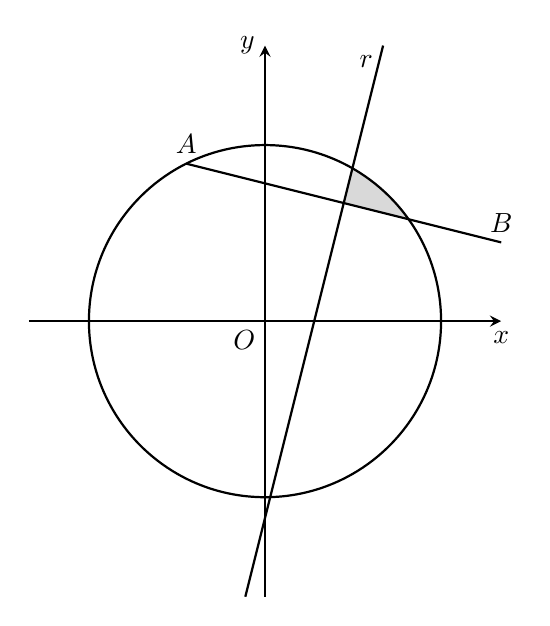
\begin{tikzpicture}
        % definir A, B e O
        \coordinate[label=below left:{$O$}] (O) at (0,0);
        \coordinate[label={$A$}] (A) at (-1,2);
        \coordinate[label={$B$}] (B) at (3,1);

        % definir pontos da mediatriz de [AB]
        \coordinate (M) at ($0.5*(A)+0.5*(B)$);
        \coordinate[rotate around={90:(M)}] (P) at ($(B)$);
        \coordinate (P1) at ($(M) + 2.5*(M)-2.5*(P)$);

        %sombreado
        \begin{scope}
            \clip(0,0) circle ({sqrt(5)});
            \filldraw[gray!30] (M)--(B)--(P);
        \end{scope}

        % desenhar circulo e retas
        \draw[thick] (O) circle ({sqrt(5)});
        
        \draw[thick] (A) -- (B);
        \draw[thick] (P1) -- (P) node[below left]{$r$};
        
        % desenhar eixos
        \draw[->, thick, >=stealth] (-3,0) -- (3,0) node[below] {$x$};
        \draw[->, thick, >=stealth] (0,-3.5) -- (0,3.5) node[left] {$y$};
    \end{tikzpicture}
\end{document}